\qrchapter{https://forgottenpillar.com/rsc/en-fp-chapter1}{Msingi wa Imani Yetu}

\egw{\textbf{Bwana ataweka nguvu mpya, katika kazi Yake} huku binadamu wakitii amri ya kwenda mbele na kutangaza ukweli. \textbf{Yeye ambaye alitangaza kwamba ukweli wake ungeangaza milele atatangaza ukweli huu kupitia wajumbe waaminifu, ambao wataipa tarumbeta sauti bainifu}. \textbf{Ukweli utashutumiwa, kudharauliwa, na kudhihakiwa; lakini kadiri utakavyohunguzwa \underline{zaidi} na kupimwa, ndivyo \underline{utakavyong'aa zaidi}}.}[SpTB02 51.1; 1904][https://egwwritings.org/read?panels=p417.260]

\egwnogap{\textbf{Kama watu, tunapaswa \underline{kusimama kidete kwenye jukwaa la ukweli wa milele} ambao umestahimili mtihani na majaribio. Tunapaswa \underline{kushikilia nguzo za hakika za imani yetu}. \underline{Kanuni za ukweli} ambazo Mungu ametufunulia \underline{ndio msingi wetu pekee wa kweli}. Zimetufanya tulivyo. Mpito wa wakati haujapunguza thamani yao. \underline{Ni juhudi za mara kwa mara za adui kuondoa ukweli huu kutoka kwa mpangilio wao}, na kuweka mahali pao \underline{nadharia potofu}. Yeye \underline{ataleta} kila kitu awezacho ili kutekeleza mipango yake ya udanganyifu. Lakini Bwana atainua watu wenye utambuzi makini, ambao watazipa kweli hizi sehemu yao katika mpango wa Mungu.}}[SpTB02 51.2; 1904][https://egwwritings.org/read?panels=p417.261]

\egwnogap{\textbf{Nimeagizwa na mjumbe wa mbinguni kwamba baadhi ya hoja katika kitabu, ‘Living Temple,’ hazifai na kwamba \underline{hoja hizi zitapotosha} akili za wale ambao hawajasimama kikamilifu juu ya \underline{kanuni za msingi} za ukweli wa sasa. Inatanguliza yale ambayo si chochote bali dhana tu kuhusiana na \underline{Umbile la Mungu na mahali uwepo wake upo}}. Hakuna mtu katika dunia hii ana haki ya kukisia juu ya swali hili. \textbf{Kadiri nadharia potofu zinavyojadiliwa, ndivyo watu watakavyojua kidogo kuhusu Mungu na ukweli unaotakasa nafsi}.}[SpTB02 51.3; 1904][https://egwwritings.org/read?panels=p417.262]

\egwnogap{Mmoja baada ya mwingine anakuja kwangu, akiniuliza \textbf{nieleze nafasi zilizochukuliwa katika ‘Living Temple.’} Ninajibu, ‘\textbf{Hazielezeki}.’ \textbf{Maoni yanayoonyeshwa hayatoi ukweli sahihi wa Mungu}. Kitabuni pote pana vifungu vya maandiko. Maandiko haya yamewekwa kwa njia ambayo kosa linafanywa kuonekana kuwa kweli. \textbf{Nadharia potofu zinawasilishwa kwa njia ya kupendeza kiasi kwamba tusipochunga, wengi watapotezwa}.}[SpTB02 52.1; 1904][https://egwwritings.org/read?panels=p417.265]

\egwnogap{\textbf{Hatuhitaji mafumbo yaliyo katika kitabu hiki}. Wale wanaoyapa sikio mafumbo haya hivi karibuni watajikuta katika nafasi ambayo adui anaweza kuzungumza nao, na kuwaongoza mbali na Mungu. Imeonyeshwa kwangu kwamba mwandishi wa kitabu hiki yuko kwenye njia ya uwongo. \textbf{Amepoteza mtazamo wa kweli halisi za \underline{wakati huu}}. Hajui hatua zake zinapoenenda. \textbf{\underline{Njia ya ukweli ipo karibu na njia ya uongo}, na njia zote mbili zinaweza kuonekana kuwa moja kwa akili ambazo hazifanyiwi kazi na Roho Mtakatifu, na ambazo, kwa hiyo, si nyepesi kutambua tofauti kati ya ukweli na uongo}.}[SpTB02 52.2; 1904][https://egwwritings.org/read?panels=p417.266]

\egwnogap{\textbf{Takriban wakati ambapo ‘Living Temple’ ilichapishwa, mbeleni mwangu mlipitishwa katika msimu wa usiku, \underline{maono yaliyoonyesha kwamba hatari fulani ilikuwa inakaribia}, na kwamba ni lazima nijitayarishe kwa \underline{kuandika mambo} ambayo Mungu amenifunulia \underline{kuhusu kanuni za msingi za imani yetu}}.}[SpTB02 52.3; 1904][https://egwwritings.org/read?panels=p417.267]

\egwnogap{Nilipewa nakala ya ‘Living Temple’ lakini ilibaki kwenye maktaba yangu, bila kusomwa. Kutoka kwa nuru niliyopewa na Bwana, \textbf{nilijua kwamba baadhi ya maoni yanayotetewa katika kitabu hicho, hazina uidhinishaji wa Mungu}, \textbf{na kwamba zilikuwa ni \underline{mtego ambao adui alitayarisha kwa ajili ya siku za mwisho}}. Nilidhani kwamba hili hakika lingetambuliwa, na kwamba haingekuwa lazima kwangu kusema chochote juu yake.}[SpTB02 52.4; 1904][https://egwwritings.org/read?panels=p417.268]


\egwnogap{Katika mgogoro uliotokea kati ya ndugu zetu \textbf{kuhusu mafundisho ya kitabu hiki}, wale waliopendelea kukisambaza walitangaza: ‘\textbf{Kina maoni yale yale ambayo Dada White amekuwa akifundisha}.’ Usemi huu uligusa moyo wangu kabisa. Nilihisi kuvunjika moyo; kwa maana \textbf{nilijua kuwa usemi huu \underline{haukuwa wa kweli}}.}[SpTB02 53.1; 1904][https://egwwritings.org/read?panels=p417.270]


\egwnogap{Mwishowe mwanangu akaniambia, ‘Mama, unapaswa kusoma angalau sehemu fulani za kitabu, upate kuona kama zinapatana na nuru ambayo Mungu amekupa.’ Akaketi chini kando yangu, na kwa pamoja \textbf{tulisoma dibaji, na sehemu kubwa ya sura ya kwanza, na pia aya katika sura nyingine}. Tulipokuwa tukisoma, nilitambua maoni yale yale ambayo nilikuwa nimeagizwa kuzungumza dhidi yao \textbf{ \underline{siku za mwanzo} za kazi yangu ya umma}. Nilipoondoka Jimbo la Maine kwa mara ya kwanza, ilikuwa ni kupitia Vermont na Massachusetts, kubeba ushuhuda dhidi ya maoni haya. \textbf{‘Living Temple’ ina alfa ya nadharia hizi. Nilijua kuwa \underline{omega ingefuata baada ya muda mfupi}; na nikatetemeka kwa ajili ya watu wetu}. \textbf{Nilijua kwamba lazima niwaonye ndugu na dada zetu wasiingie katika mabishano \underline{juu ya uwepo na Umbile la Mungu}}. \textbf{Kauli zilizotolewa katika ‘Living Temple’ \underline{kuhusu suala hili si sahihi}}. Maandiko yaliyotumika kuthibitisha mafundisho yaliyowekwa hapo yametumika vibaya.}[SpTB02 53.2; 1904][https://egwwritings.org/read?panels=p417.271]

\egwnogap{\textbf{Ninalazimika kukana madai kwamba mafundisho ya ‘Living Temple’ yanaweza kudumishwa kwa maandishi yangu}. \textbf{Kunaweza kuwa katika kitabu hiki maneno yanayopatana na maandishi yangu}. \textbf{Na kunaweza kuwa katika maandishi yangu taarifa nyingi ambazo, zikichukuliwa kutoka kwa muktadha wao, na kufasiriwa kulingana na mawazo ya mwandishi wa ‘Living Temple’, zitaonekana kana kwamba zinapatana na mafundisho ya kitabu hiki.} Hili linaweza kutia nguvu madai kwamba mafundisho katika ‘Living Temple’ yanapatana na maandishi yangu. \textbf{Lakini Mungu azuie dhana hii isiimarike}.}[SpTB02 53.3; 1904][https://egwwritings.org/read?panels=p417.272]

\egwnogap{\textbf{Wachache wanaweza kutambua matokeo ya kupa sikio mafundisho ya uwongo yanayotetewa sasa}. \textbf{Lakini Bwana ameinua pazia na \underline{kunionyesha matokeo ambayo yatafuata}}. \textbf{Nadharia za umizimu \underline{kuhusu Umbile la Mungu}, zikifuatwa hadi kwenye hitimisho, hufagia mbali ukristo wote}. \textbf{Hudhalilisha nuru ambayo Kristo alikuja nayo kutoka mbinguni na kumpa Yohana ili awape watu wake. Hufundisha kwamba matukio yaliyo mbele yetu si ya umuhimu wa kutosha wa kupewa umakini maalum. Hudhalilisha ukweli wa asili ya mbinguni, \underline{na kuwaibia watu wa Mungu uzoefu wao wa zamani}, na kuwapa badala yake sayansi ya uwongo}.}[SpTB02 54.1; 1904][https://egwwritings.org/read?panels=p417.275]

\egwnogap{\textbf{Katika maono} ya usiku nilionyeshwa waziwazi kwamba \textbf{mafundisho haya} yametazamwa na wengine kama \textbf{kweli kuu} \textbf{ambazo zinapaswa \underline{kuletwa}} na kufanywa kuwa maarufu katika wakati uliopo. \textbf{Nilionyeshwa \underline{jukwaa}, lililoimarishwa na \underline{mbao ngumu},—kweli za Neno la Mungu}. \textbf{Mtu fulani aliye juu katika kazi ya matibabu alikuwa akimwongoza mtu huyu na mtu huyo kulegeza mbao zinazoshikilia jukwaa hili}. Kisha nikasikia sauti ikisema, ‘Wako wapi walinzi wanaopaswa kusimama juu ya kuta za Sayuni? Je! wamelala? \textbf{\underline{Msingi huu ulijengwa na Mfanyakazi Mkuu}, na \underline{utasimama} dhoruba na tufani. Je, watamruhusu mtu huyu \underline{kuwasilisha mafundisho} \underline{yanayopinga uzoefu wa awali} wa watu wa Mungu? Wakati umefika wa kuchukua hatua maalum}.’}[SpTB02 54.2; 1904][https://egwwritings.org/read?panels=p417.276]

\egwnogap{\textbf{Adui wa roho ametaka kuleta dhana kwamba matengenezo makubwa yangetukia kati ya Waadventista Wasabato, na kwamba matengenezo haya yangehusu kutoa mafundisho ambayo yanasimama kama nguzo za imani yetu, na kuanza mikakati ya kujipanga upya}. \textbf{Je, matengenezo haya yangefanyika, \underline{matokeo yake yangekuwa nini}?} \textbf{\underline{Kanuni za ukweli} ambazo Mungu katika hekima yake amelipatia kanisa la masalio, \underline{zingetupwa}}. \textbf{Dini yetu ingebadilishwa}. \textbf{\underline{Kanuni za msingi} ambazo zimedumisha kazi hiyo kwa miaka hamsini iliyopita \underline{zingehesabiwa kama makosa}}. \textbf{Shirika mpya lingeanzishwa}. \textbf{Vitabu vya agizo jipya vingeandikwa}. \textbf{Mfumo wa falsafa ya kiakili ungeanzishwa}. Waanzilishi wa mfumo huu wangeenda katika miji, na kufanya kazi ya ajabu. Sabato, bila shaka, ingechukuliwa kuwa nyepesi, \textbf{kama vile Mungu aliyeiumba}. Hakuna kitu kingeruhusiwa kusimama kwenye njia ya mfumo huu mpya. \textbf{Viongozi wangefundisha kwamba wema ni bora kuliko uovu, lakini kwa kuwa Mungu ameondolewa, wangeweka utegemezi wao kwa nguvu za kibinadamu, ambazo, bila Mungu, hazina thamani}. \textbf{Msingi wao ungejengwa juu ya mchanga, na dhoruba na tufani zingefagia muundo huo}.}[SpTB02 54.3; 1904][https://egwwritings.org/read?panels=p417.277]

\egwnogap{Nani mwenye mamlaka ya kuanzisha harakati hiyo? \textbf{Tuna Biblia zetu}. \textbf{Tuna uzoefu wetu, unaothibitishwa na utendaji wa kimiujiza wa Roho Mtakatifu}. \textbf{Tuna ukweli ambao hautaki mapatano ya kuafikiana}. \textbf{\underline{Je, hatutakataa vyote ambavyo haviafikiani na ukweli huu}}?}[SpTB02 55.1; 1904][https://egwwritings.org/read?panels=p417.280]

\egwnogap{Nilichelea na kuchelewa kutuma yale ambayo Roho wa Bwana alinisukuma kuandika. \textbf{Sikutaka kulazimishwa kuwasilisha ushawishi wa kupotosha wa mafundisho haya ya uwongo. Lakini kwa majaliwa ya Mungu, lazima nikutane na makosa ambayo yamekuwa yakiingia}.}[SpTB02 55.2; 1904][https://egwwritings.org/read?panels=p417.281]

\egwnogap{Muda mfupi kabla \textbf{sijatuma shuhuda kuhusu \underline{juhudi za adui kudhoofisha msingi wa imani yetu} kwa njia ya \underline{uenezaji wa nadharia potofu}}, nilikuwa nimesoma tukio kuhusu meli iliyokaribia kukutana na barafu, na anga ilikuwa na ukungu. Kwa usiku kadhaa nililala kidogo. Nilionekana nimeinama chini kama mkokoteni chini ya miganda. Usiku mmoja tukio liliwasilishwa wazi mbele yangu. Meli ilikuwa juu ya maji, katika ukungu mzito. Ghafla mlinzi akapaza sauti, ‘Barafu iko mbele!’ Hapo, mbele ya meli, kulikuwa na barafu iliyokuwa ndefu kuliko meli. Sauti yenye mamlaka ilipaza sauti, ‘Kutana nayo!’ Hakukuwa na kusitasita hata kidogo. Ulikuwa wakati wa kuchukua hatua ya mara moja. Mhandisi aliweka mvuke kamili, na mtu aliyekuwa kwenye gurudumu akaiongoza meli moja kwa moja hadi kwenye kilima cha barafu, akakipoga kwa kishindo. Mshtuko wa kutisha ulitokea, na barafu ikavunjika vipande vipande, ikaangukia sitaha kwa sauti kama ya radi. Abiria walitikiswa kwa nguvu ya mgongano, lakini hakuna aliyekufa. Meli hiyo ilijeruhiwa, japo kwa kiwango inayoweza kurekebishwa. Ilirudi kutoka kwa pambano huku ikitetemeka kutoka shina hadi tezi, kama kiumbe hai. Kisha ikasonga mbele kuendelea na njia yake.}[SpTB02 55.3; 1904][https://egwwritings.org/read?panels=p417.282]

\egwnogap{Nilijua maana ya niliyoona. \textbf{Nilikuwa na maagizo yangu}. Nilisikia maneno, kama sauti kutoka kwa Kapteni wetu, ‘\textbf{Kutana nayo}!’ Nilijua wajibu wangu ulikuwa ni nini, na kwamba hapakuwa na muda wa kupoteza. Wakati wa kuchukua hatua ulikuwa umefika. \textbf{Ni lazima bila kuchelewa kutii amri, ‘Kutana nayo!’}}[SpTB02 56.1; 1904][https://egwwritings.org/read?panels=p417.285]

\egwnogap{Usiku huo niliamka saa saba, nikaandika haraka kadri mkono wangu ulivyoniwezesha. Kwa siku chache zilizofuata nilifanya kazi mapema na jioni hata kuchelewa, \textbf{nikitayarishia watu wetu maagizo niliyopewa \underline{kuhusu makosa} yaliyokuwa \underline{yakiingia} kati yetu}.}[SpTB02 56.2; 1904][https://egwwritings.org/read?panels=p417.286]

\egwnogap{\textbf{Nimekuwa nikitumaini kwamba kungekuwa na mageuzi ya kina, na kwamba \underline{kanuni} ambazo tulizipigania \underline{siku za kwanza}, na ambazo zilitolewa kwa nguvu za Roho Mtakatifu, \underline{zingedumishwa}}.}[SpTB02 56.3; 1904][https://egwwritings.org/read?panels=p417.287]

\egwnogap{\textbf{Wengi wa watu wetu hawatambui \underline{jinsi kwa udhabiti} msingi wa imani yetu uliwekwa}. \textbf{Mume wangu, Mzee Joseph Bates, Baba Pierce, Mzee Edson, na wengine ambao walikuwa makini, waungwana, na wa kweli, walikuwa miongoni mwa wale ambao, baada ya muda kupita, 1844, walitafuta ukweli kama hazina iliyofichwa}. Nilikutana nao, tukasoma na kuomba kwa bidii. Mara nyingi tulibaki pamoja hadi usiku sana, na wakati mwingine mpaka kukakucha, tukiomba kwa ajili ya nuru na tukijifunza neno. Tena na tena hawa ndugu walikuja pamoja kujifunza Biblia, ili wapate kujua maana yake, na kuwa tayari kuufundisha kwa nguvu. Walipofikia hatua katika funzo lao ambapo walisema, ‘Hatuwezi zaidi,’ Roho wa Bwana angenijia, ningepata maono, na ningepewa maelezo ya wazi ya vifungu tulivyokuwa tukijifunza, pamoja na maagizo ya jinsi tunapaswa kufanya kazi na kufundisha kwa ufanisi. Kwa njia hiyo nuru ilitolewa ambayo ilitusaidia sisi kuelewa maandiko kuhusu Kristo, utume wake, na ukuhani Wake. \textbf{Mstari wa ukweli unaoenea kutoka wakati huo hadi wakati ambapo tutaingia katika jiji la Mungu, uliwekwa wazi kwangu, na nikawapa wengine maagizo ambayo Bwana alinipa}.}[SpTB02 56.4; 1904][https://egwwritings.org/read?panels=p417.288]


\begin{figure}
    \centering
    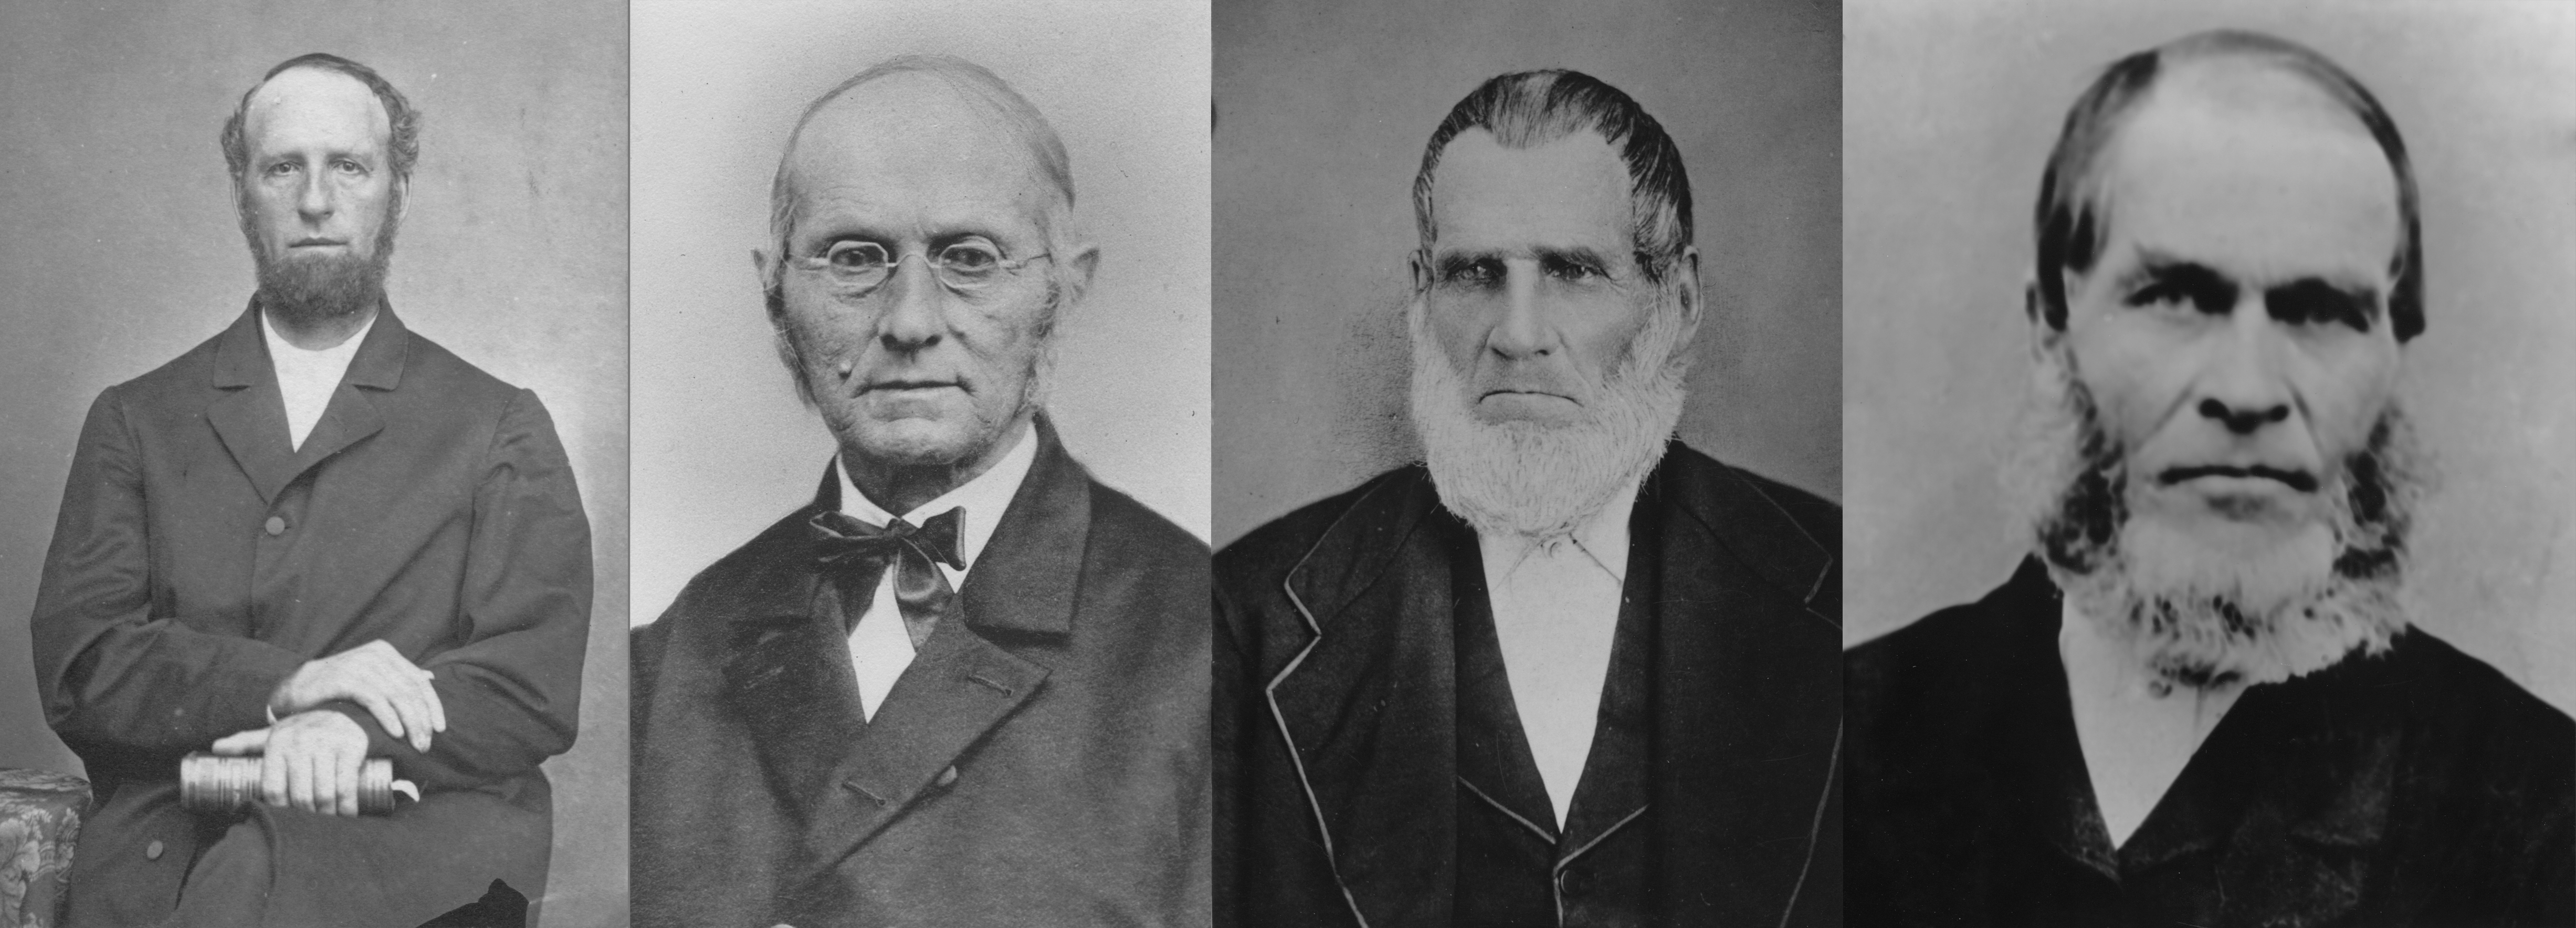
\includegraphics[width=1\linewidth]{images/james-white-joseph-bates-stephen-pierce-hiram-edson.jpg}
    \caption*{James White, Joseph Bates, Stephen Pierce, Hiram Edson}
    \label{fig:pioneers}
\end{figure}


\begin{figure}
    \centering
    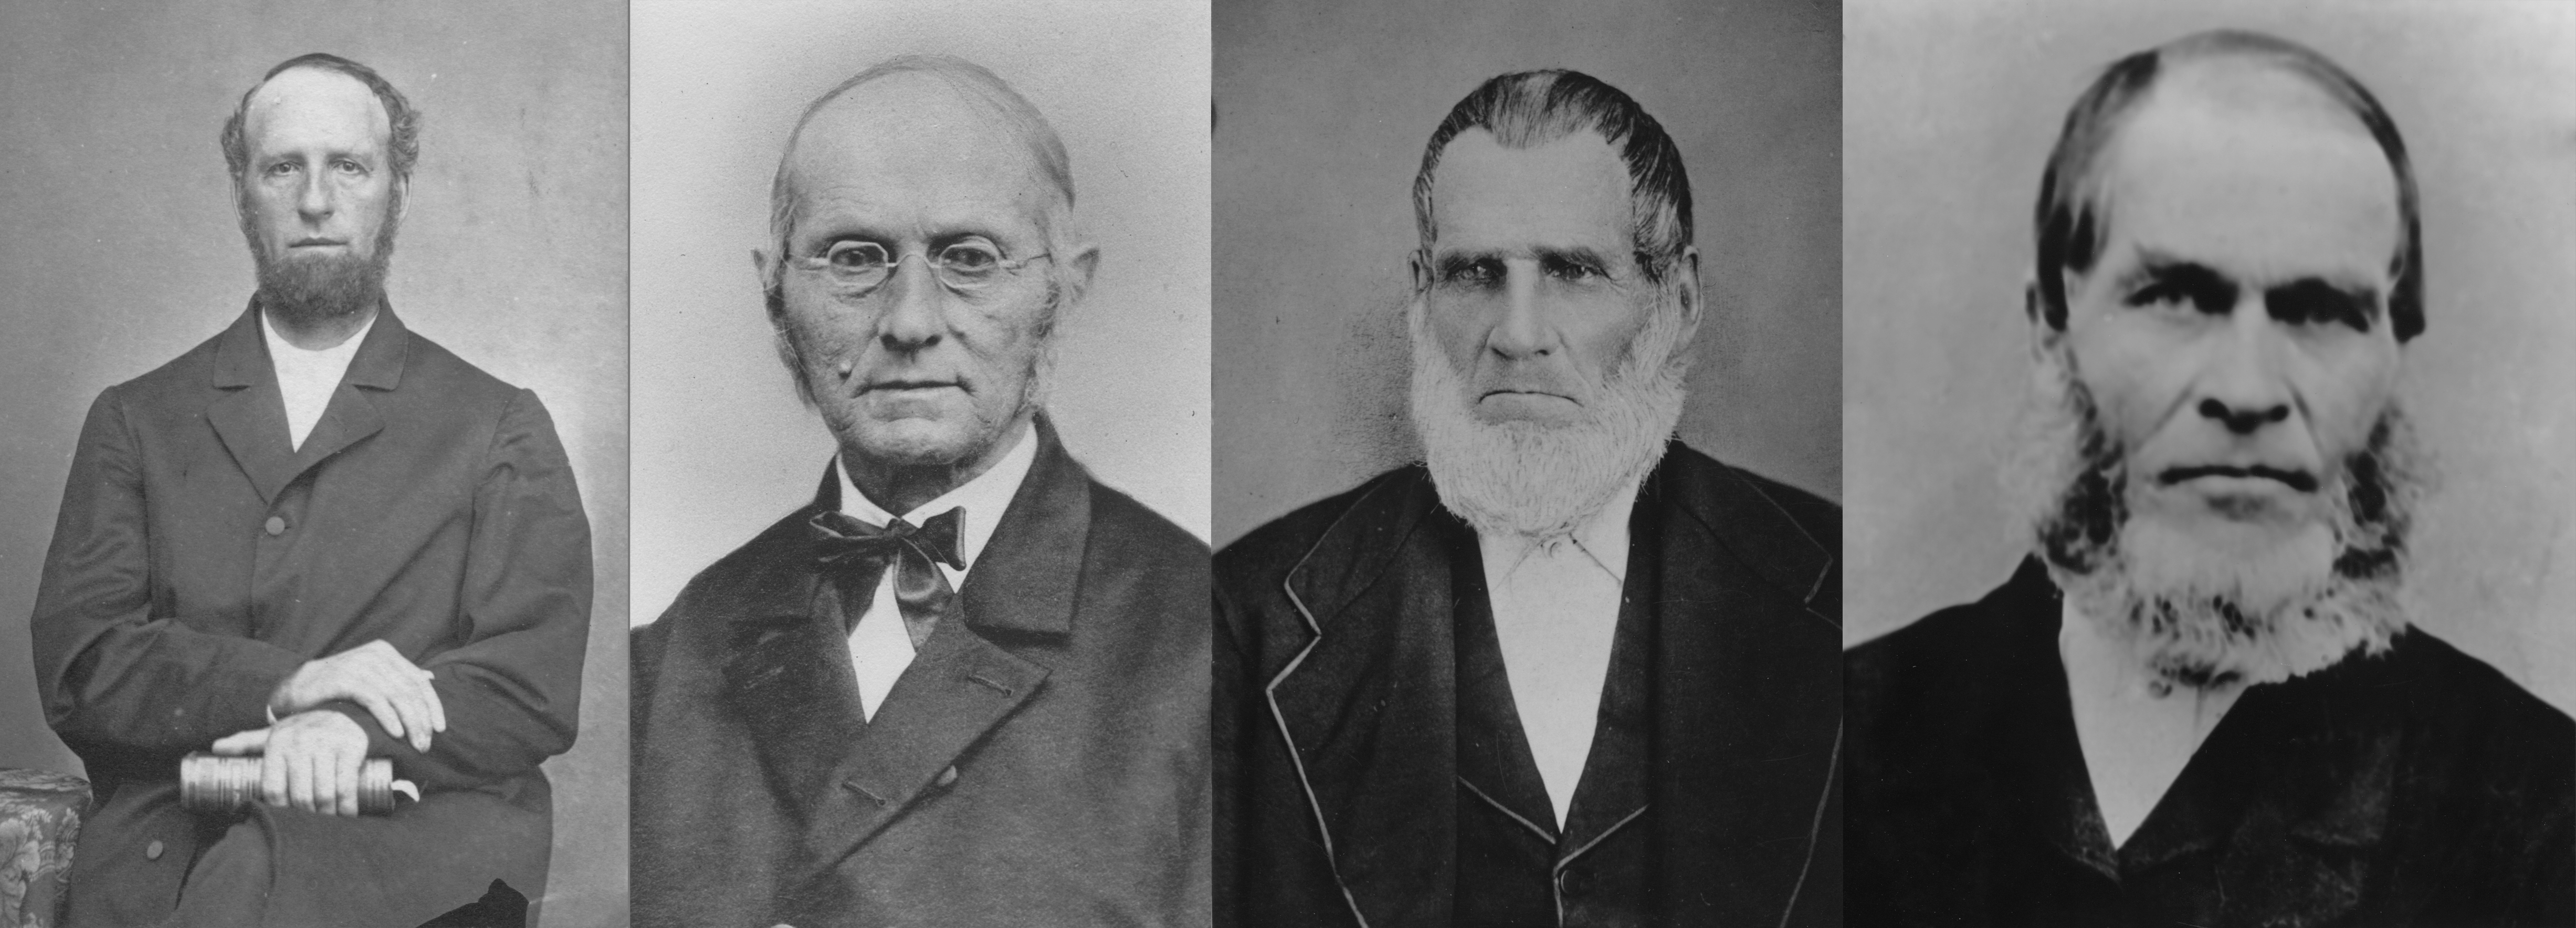
\includegraphics[width=1\linewidth]{images/james-white-joseph-bates-stephen-pierce-hiram-edson.jpg}
    \caption*{James White, Joseph Bates, Stephen Pierce, Hiram Edson}
    \label{fig:pioneers}
\end{figure}


\egwnogap{Wakati huu wote sikuweza kuelewa hoja za ndugu zangu. Akili yangu ilikuwa imefungwa, na sikuweza kuelewa maana ya maandiko tuliyokuwa tukisoma. Hii ilikuwa mojawapo ya huzuni kubwa zaidi ya maisha yangu. \textbf{Nilikuwa katika hali hii ya akili mpaka \underline{pointi kuu za imani yetu} zikawekwa wazi kwa akili zetu, kwa kupatana na neno la Mungu}. Ndugu walijua kwamba wakati ambapo sikuwa katika maono, singeweza kuelewa mambo haya, na wakakubali kama nuru ya moja kwa moja kutoka mbinguni, mafunuo yaliyotolewa.}[SpTB02 57.1; 1904][https://egwwritings.org/read?panels=p417.291]

\egwnogap{Kwa miaka miwili au mitatu akili yangu iliendelea kufungwa hata nisielewe Maandiko. Katika shughuli za kazi zetu, mume wangu na mimi tulimtembelea Baba Andrews, ambaye alikuwa anateseka sana kutokana na inflammatory rheumatism. Tulimuombea. Niliweka mikono yangu juu ya kichwa chake, na kusema, ‘Baba Andrews, Bwana Yesu akuponya.’ Akaponywa papo hapo. Akainuka, na kuzunguka zunguka chumbani, akimsifu Mungu, na kusema, ‘Sijawahi kuiona kwa njia hii awali. Malaika wa Mungu wako katika chumba hiki.’ Utukufu wa Bwana ukafunuliwa. Mwanga ulionekana kuangaza nyumba nzima, na mkono wa malaika uliwekwa juu ya kichwa changu. Kutoka wakati huo nimeweza kuelewa neno la Mungu.}[SpTB02 57.2; 1904][https://egwwritings.org/read?panels=p417.292]

\egwnogap{\textbf{Ni ushawishi gani ambao unaweza kusababisha watu katika hatua hii ya historia yetu kufanya kazi katika njia ya kichinichini, yenye nguvu za\underline{kubomoa msingi wa imani yetu},—msingi ambao uliwekwa mwanzoni mwa kazi yetu kwa kujifunza neno kwa maombi na kwa ufunuo? Juu ya \underline{msingi huu} tumekuwa tukijenga kwa \underline{miaka hamsini iliyopita}. Hivyo unashangaa kwamba ninapoona mwanzo wa kazi ambayo \underline{itaondoa baadhi ya nguzo za imani yetu}, ninalo la kusema? Ni lazima nitii amri, ‘Kutana nayo!’}}[SpTB02 58.1; 1904][https://egwwritings.org/read?panels=p417.295]

\egwnogap{Nina hisia nzito kwa Dkt. Kellogg. Kwa miaka mingi nimejaribu sana kumshikilia. Neno la Mungu kwangu sikuzote limekuwa, ‘Unaweza kumsaidia.’ Wakati fulani mimi huamshwa usiku, na, nikiamka, ninatembea chumbani, nikiomba: ‘Ee Bwana, mshikilie Dk. Kellogg. Usimruhusu kwenda. Muweke imara. Mpake macho yake dawa ya macho ya mbinguni, ili aone mambo yote waziwazi.’ Usiku baada ya usiku nimelala macho, nikichunguza jinsi nitakavyomsaidia. Kwa bidii na mara nyingi nimeomba kwamba Bwana asiweze kumruhusu kugeuka kutoka kwa ukweli wa kutakasa. Huu ndio mzigo unaonilemea, - hamu kuwa atazuiliwa asifanye makosa ambayo yataumiza nafsi yake na \textbf{kudhuru kazi ya ukweli wa sasa}. Lakini kwa muda fulani matendo yake yamedhihirisha kuwa roho ya ajabu inamtawala. Bwana atachukua jambo hili katika mikono yake mwenyewe. Yanipasa kutangaza jumbe za maonyo ambazo Mungu hunipa kutangaza, na kisha kumwachia Bwana matokeo. \textbf{Ni lazima sasa niwasilishe jambo hili ili watu wa Mungu wasitekwe nyara}.}[SpTB02 58.2; 1904][https://egwwritings.org/read?panels=p417.296]

\egwnogap{\textbf{Sisi ni watu wa Mungu wanaozishika amri zak. Kwa miaka hamsini iliyopita kila uzushi umeletwa juu yetu, ili kuziba akili zetu tusielewe mafundisho ya neno},\textbf{—hasa kuhusu huduma ya Kristo katika patakatifu pa mbinguni, na ujumbe wa mbinguni kwa siku hizi za mwisho, kama ulivyotolewa na malaika wa sura ya kumi na nne ya Ufunuo}. \textbf{Jumbe za aina yote zimeletwa kwa Waadventista Wasabato, kuchukua mahali pa ile kweli ambayo, \underline{hatua kwa hatua}, imetafutwa kwa kujifunza kwa maombi, na kushuhudiwa na uweza wa Bwana utendao miujiza}. \textbf{Lakini \underline{alama za njia} \underline{ambazo zimetufanya tuwe vile tulivyo}, \underline{zinapaswa kuhifadhiwa}, na \underline{zitahifadhiwa}, kama vile Mungu ameonyesha kupitia kwa neno lake na ushuhuda wa Roho wake}. \textbf{Anatuita \underline{tushikilie kwa uthabiti}, kwa mshiko wa imani, \underline{kanuni za msingi} ambazo \underline{msingi wake ni mamlaka isiyotiliwa shaka}}.}[SpTB02 59.1; 1904][https://egwwritings.org/read?panels=p417.299]

Kulikuwa na haja ya dharura ya kuonya kanisa kuhusu kazi ya adui ya kung'oa msingi wa imani yetu. Kulikuwa na dharura ya kulikumbusha kanisa ni nini inayojumuisha msingi wa kweli wa imani ya Waadventista Wasabato. Inaonekana kwamba Waadventista Wasabato, wa wakati huo, walikuwa wamesahau \egwinline{njia ambayo Bwana ametuongoza, na mafundisho Yake katika historia yetu iliyopita.}[LS 196.2; 1915][https://egwwritings.org/read?panels=p41.1083]

\egw{Ni ushawishi gani ambao unaweza kusababisha watu katika hatua hii ya historia yetu kufanya kazi katika njia ya kichinichini, yenye nguvu \textbf{kubomoa msingi wa imani yetu},—msingi ambao uliwekwa \textbf{mwanzoni mwa kazi yetu} kwa kujifunza neno kwa maombi na kwa ufunuo? Juu ya \textbf{msingi huu} tumekuwa tukijenga kwa \textbf{miaka hamsini iliyopita}. Hivyo unashangaa kwamba ninapoona mwanzo wa kazi ambayo \textbf{itaondoa baadhi ya nguzo za imani yetu}, nina la kusema? Ni lazima nitii amri, ‘\textbf{Kutana nayo}!’}[SpTB02 58.1; 1904][https://egwwritings.org/read?panels=p417.295]


Ni nini ambacho Dada White aliamrishwa akutane nacho?

\egwinline{Takriban wakati ambapo ‘Hekalu Hai’ ilichapishwa} katika msimu wa usiku alipokea \egwinline{maelezo yanayoonyesha kwamba hatari fulani ilikuwa inakaribia,} na kwamba lazima \egwinline{ajitayarishe kwa hiyo kwa kuandika mambo ambayo Mungu amemfunulia} kuhusu \egwinline{\textbf{kanuni za msingi za imani yetu}.}

Alifunuliwa \egwinline{na mjumbe wa mbinguni kwamba baadhi ya hoja zilizo katika kitabu, ‘Hekalu Hai’, hazina maana na kwamba \textbf{mawazo haya yangepotosha} akili za wale ambao hawajathibitishwa kikamilifu juu ya \textbf{kanuni za msingi} za ukweli wa sasa.}


Kwa hivyo, shida halisi ya kitabu, “Hekalu Hai” ilikuwa nini?


Ikiwa wewe ni msomi, au mwanahistoria wa Kiadventista, au mwanatheolojia, au mwanafunzi tu wa theolojia, kabla ya kutoa jibu la moja kwa moja na kusema kwamba tatizo lilikuwa pantheism, tungependa kukuelekeza kwenye maandishi. Dada White alizungumzia kwa uwazi suala la msingi wa tatizo akisema kwamba “Hekalu Hai,” \egwinline{inatanguliza yale ambayo ni dhana tu kuhusu \textbf{ubinafsi wa Mungu} na \textbf{mahali uwepo wake upo}.}


Hatukatai shida ya pantheism ya kitabu, lakini tunataka kugeuza makini kutoka kwa kosa la Kellogg hadi kwenye nuru ambayo Mungu ametoa. Kuna njia mbili za kukabiliana na shida ya Kellogg. Njia moja ni kuangazia fundhisho la pantheism, na njia nyingine ni kuangazia \egwinline{\textbf{ubinafsi wa Mungu} na \textbf{mahali uwepo wake upo}}. Njia moja ni kusoma kosa, na njia nyingine ni kusoma Ukweli. Njia moja ni kupasua giza na njia nyingine ni kunywa kutoka kwenye chemchemi ya ukweli. Tunachagua la mwisho, na kwa sababu hii, kitabu hiki kimetengwa kutoka kwa mamia ya vitabu vingine vilivyoandikwa kuhusu mgogoro wa Kellogg. Mada ya kitabu hiki sio pantheism, au kosa lingine lolote, bali ukweli na kile ambacho Mungu amefichua kuhusu Umbile lake na mahali ambapo uwepo wake upo. Huu ndio ulikuwa suala halisi la uchapishaji wa Kellogg.


Tunaamini kuwa ni hatari kubwa kusoma na kuchambua makosa kwa sababu makosa husababisha udanganyifu. Tatizo la udanganyifu ni kwamba tunaweza kudanganywa bila kujua tunadanganywa! Tunaamini kabisa kwamba Ellen White alikuwa nabii wa Mungu na kwamba yeye alikuwa akipokea Nuru kutoka kwa Mungu \bible{aliye nuru na ndani yake hamna giza hata kidogo}[1 Yohana 1:5]. Kwa hiyo, hatutarajii Dada White kueleza kosa liliko katika kitabu, “Hekalu Hai”. Wengi walikuwa wakimjia, wakimwomba \egwinline{aeleze nafasi zilizochukuliwa katika ‘Hekalu Hai.’} Yeye akajibu, \egwinline{Hayaelezeki}. Lengo lake halikuwa kuchambua kosa bali kuangaza Ukweli juu ya \emcap{Umbile la Mungu} na mahali ambapo uwepo wake upo. Kwa hivyo, alikuwa akielekeza nyuma kwa kweli ambazo juu yazo, Mungu alianzisha Kanisa la Waadventista Wasabato. Kweli hizi zimekuwa msingi wa imani yetu. Kweli hizi tulipewa katika siku zetu za mwanzo. Kwa kugeuza mawazo yetu kutoka kwa Umbile la Mungu hadi kwenye pantheism, tunapoteza nafasi ya kukumbuka \egwinline{\textbf{jinsi Bwana ametuongoza}, na \textbf{mafundisho Yake} katika \textbf{historia yetu}}. Kwa mtazamo huu, tunaelezea wasiwasi wetu juu ya mgogoro wa Kellogg na mtazamo wake wa pantheism, kwa sababu \egwinline{njia ya ukweli ipo karibu na njia ya makosa, na njia zote mbili zinaweza kuonekana kuwa moja}; suluhisho la hilo ni \egwinline{kuimarishwa kabisa juu ya \textbf{kanuni za msingi} za ukweli wa sasa}. Mahali pengine, Dada White alitia nguvu kanuni hii.


\egw{Shetani hajalala usingizi kamwe; yuko macho na anacheza mchezo wa maisha kwa ajili ya roho za watu wa Mungu. Atawajia kwa kujipendekeza kwa kila namna, kwa matumaini ya kuwaongoza kutoka kwa utiifu wao. Anatamani kutoa umakini wao kutoka kwa \textbf{masuala muhimu} awaelekeze kwa \textbf{nadharia za uongo}.}[Ms132-1903.42; 1904][https://egwwritings.org/read?panels=p9056.56]


Kwa hivyo, tuelekeze mawazo yetu kwenye suala halisi badala ya nadharia potofu.


% The Foundation of our Faith

\begin{titledpoem}
    \stanza{
        Pillars of truth, laid with care, \\
        By pioneers who sought in prayer. \\
        Principles firm, the Lord's design, \\
        A platform strong, for all time.
    }

    \stanza{
        Beware the subtle shifts that call, \\
        To change what should not change at all. \\
        Our identity, in these we find, \\
        God's revelations to mankind.
    }

    \stanza{
        Stand fast upon this solid ground, \\
        Where wisdom and God's light abound. \\
        Defend these truths with all your might, \\
        For in them shines eternal light.
    }
\end{titledpoem}


% The Foundation of our Faith

\begin{titledpoem}
    \stanza{
        Pillars of truth, laid with care, \\
        By pioneers who sought in prayer. \\
        Principles firm, the Lord's design, \\
        A platform strong, for all time.
    }

    \stanza{
        Beware the subtle shifts that call, \\
        To change what should not change at all. \\
        Our identity, in these we find, \\
        God's revelations to mankind.
    }

    \stanza{
        Stand fast upon this solid ground, \\
        Where wisdom and God's light abound. \\
        Defend these truths with all your might, \\
        For in them shines eternal light.
    }
\end{titledpoem}
